\providecommand{\main}{..}
\documentclass[\main/main]{subfiles}
\setboolean{isMain}{false}

\begin{document}

\title{Report for 2024/07/30}
\author{Hiroki Hamaguchi}
\maketitle

\section{CG-Newton method}

On the last time meeting, I have implemented the CG-Newton (I named it) method, non-linear conjugate gradient method with Newton's method based line search, and showed the result of the numerical experiment.
Although I'm quite interested in this topic, since I couldn't find the corresponding method in literature, I temporarily suspended the research on this topic.

According to Takahashi-san, this method might be related to \href{https://link-springer-com.utokyo.idm.oclc.org/article/10.1007/s10107-007-0170-0}{A coordinate gradient descent method for nonsmooth separable minimization}, which adopt the following line search method (I modified little bit):
\begin{screen}
  Choose $\alpha_{\mathrm{init}}$ and let $\alpha$ be the largest element of $\{ \alpha_{\mathrm{init}} \beta^i \}_{i}$ satisfying
  \begin{equation*}
    f(x+\alpha d) \leq f(x) + \alpha \sigma \qty(\grad f(x)^\top d+ \frac{1}{2} d^\top \grad^2 f(x) d).
  \end{equation*}
\end{screen}
Although this is not completely the same as the line search method I implemented, I think this is quite suggestive.
I implemented as $\alpha_{\mathrm{init}} = -\frac{d^\top \grad f(x)}{d^\top \grad^2 f(x) d}$ with normal Armijo rule, but in analysis $\alpha_{\mathrm{init}}$ doesn't affect the convergence rate. Thus, we need to prove that the obtained $\alpha$ satisfies stronger condition than the normal Armijo rule like above one.
Let us only consider the case of $f$ is convex and backtracking will not occur. Since
\begin{align*}
  f(x+\alpha d) - f(x) & \simeq \alpha \grad f(x)^\top d + \frac{\alpha^2}{2} d^\top \grad^2 f(x) d \\
                       & = -\frac{(d^\top \grad f(x))^2}{2d^\top \grad^2 f(x) d},
\end{align*}
we can expect that
\begin{equation*}
  f(x_{k+1}) - f(x_k) \leq -\frac{(d_k^\top \grad f(x_k))^2}{2d_k^\top \grad^2 f(x_k) d_k}.
\end{equation*}
However, I don't have any idea what it means and how to utilize it in the analysis.
It might necessary to consider the smoothness of $\nabla^2 f$ or something like that.

\section{Graph Drawing}

I'm sorry for sudden topic change, but I'm currently quite interested in the graph drawing problem. Firstly, let me explain why I'm interested in this topic.

On the last time meeting, I said that Random Subspace Method does work well for a narrow valley, and thus I proposed the CG-Newton method.
But based on Prof.Takeda's advise, I considered what kind of problems can be well solved by Random Subspace Method, and realized that Random Subspace Method is very suitable for the problem with separable variable $X = (x_1, x_2, \dots, x_n) \quad (x_i \in \bbR^2)$, i.e., the graph drawing problem, which is I'm very interested in from years ago.
(Actually, one of the candidates for my graduation thesis theme was about graph drawing.)

\begin{mini*}
  {X}{\sum_{i<j} f(x_i,x_j)}{}{}
\end{mini*}

As you know, stochastic gradient decent works well for the separable problem ($f=\sum_i f_i$), and separableness of $X = (x_1, x_2, \dots, x_n) (x_i \in \bbR^2)$ is corresponding to this property.

Let us consider the case a random matrix $P$ is a permutation matrix like, which is a practical situation. Then, the separableness of $X$ is necessary to terminate the algorithm in a few step.

\begin{figure}[H]
  \centering
  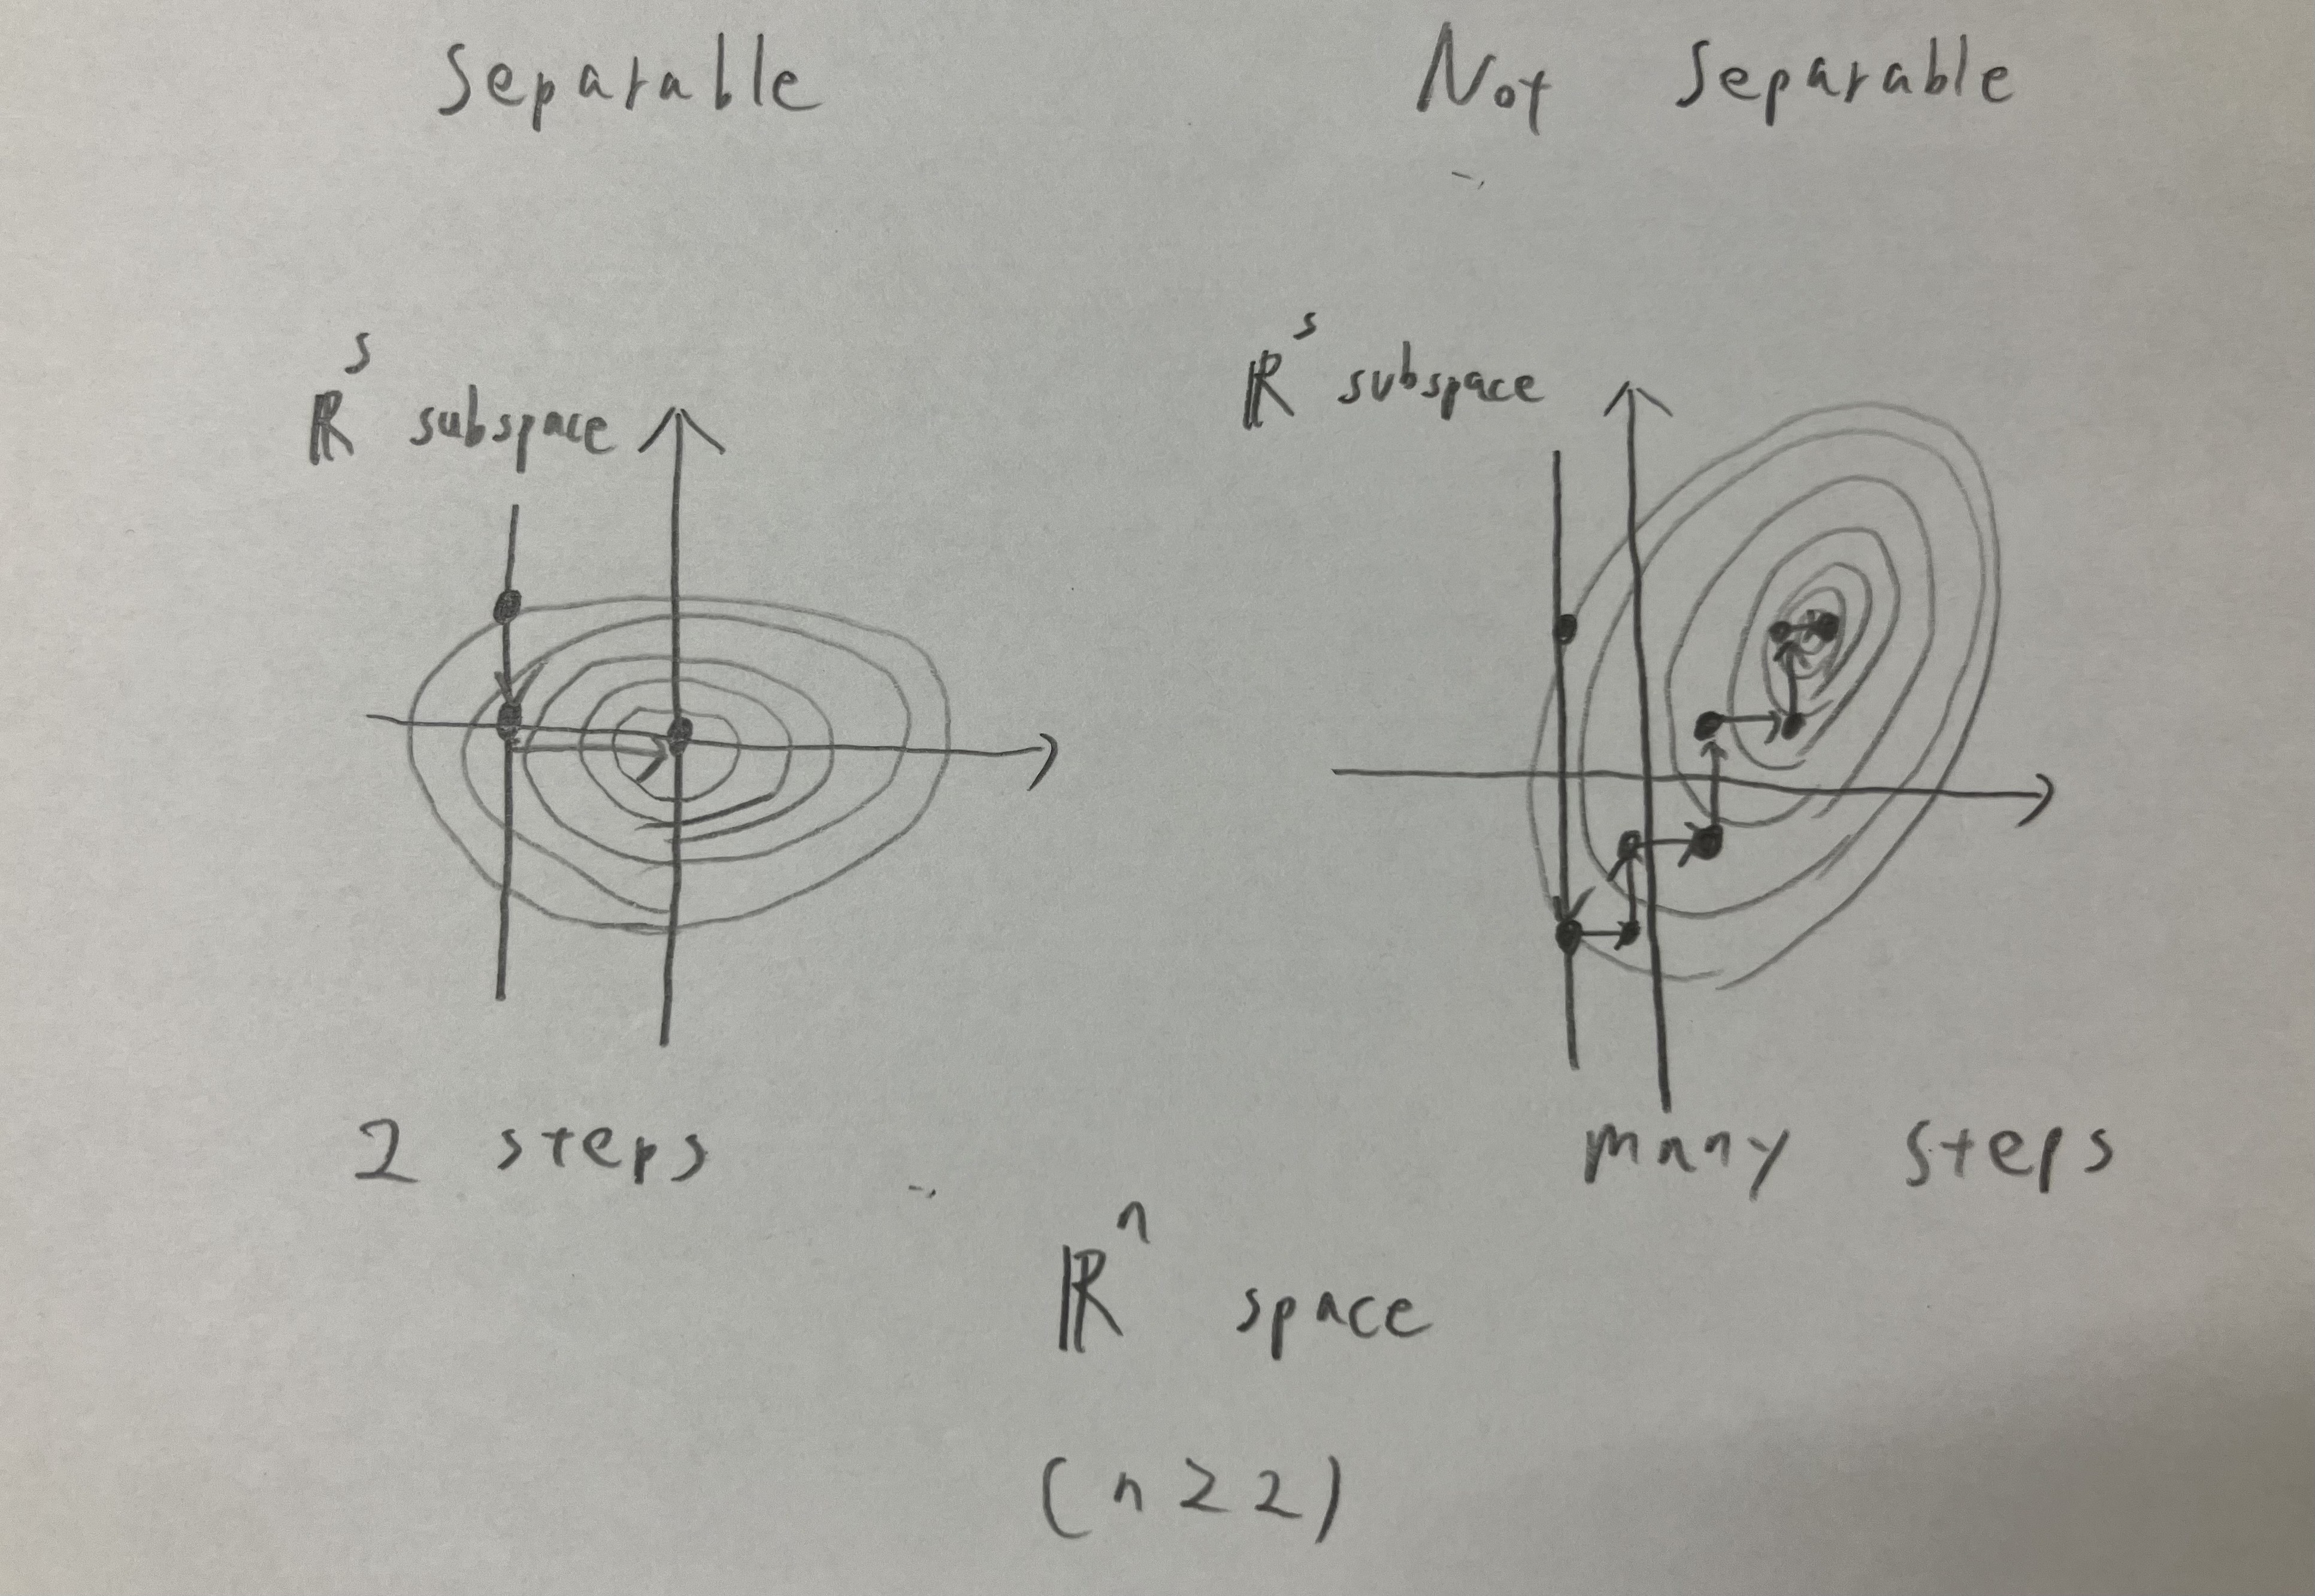
\includegraphics[width=\columnwidth]{separableX.jpg}
\end{figure}

\end{document}